\documentclass[conference]{IEEEtran}
\usepackage{cite}
\usepackage[pdftex]{graphicx}
  \graphicspath{{img/}}
  \DeclareGraphicsExtensions{.png,.jpg}
\usepackage{fixltx2e}
\usepackage{url}

\begin{document}


\title{Crypton: Zero-Knowledge Application Framework}

\author{
  \IEEEauthorblockN{Cam Pedersen}
  \IEEEauthorblockA{Engineer, Crypton\\ cam@spideroak.com}
  \and
  \IEEEauthorblockN{David Dahl}
  \IEEEauthorblockA{Director, Crypton\\ ddahl@spideroak.com}
}

\maketitle

\begin{abstract}
Applications intended to work on multiple devices or those that
store large enough amounts of data must save their data to a backend server
rather than locally. Privacy of users is typically only protected on the wire
with SSL or on the backend with an encrypted database. This leaves user data
and communications open to malicious server operators or attackers.
Application developers may easily fall into cryptographic
mistakes if they attempt to build on primitives themselves.

Crypton uses end-to-end encryption, provides application developers
with high-level APIs for user accounts, robust data storage, and
sharing information between users. We detail the framework's cryptographic
structure and its implementation architecture.
\\
\\
Project homepage: https://crypton.io
\end{abstract}

\section{Introduction}
Users' concern for the privacy of their data has become widespread
after numerous data leaks and revelations of wide spread government spying\cite{spying}.
Applications built upon zero-knowledge principals have a competitive
advantage in an emulous market. Additionally, as a service operator,
it is inherently responsible to protect users' data from intrusions
by yourself or an adversary.

Crypton is a unique way to build applications, primarily because it
makes it simple for developers to store data with a server in such a way
that the server doesn't know what that data contains.
Additionally, all Crypton-based applications are built solely on the client,
and the server acts only as a smart pipe to the database to store and retrieve data
for authenticated users. A side effect of this architecture is that working with
the framework is not dissimilar to using a "backend as a service".

\subsection{Motivation}
Moving forward from the success of SpiderOak's desktop backup client,
the logical progression is to use its Zero-Knowledge concepts in new ways -
specifically in communications applications popular on mobile devices
and desktop computers. Internet users today are tracked in unprecedented
ways by the advertising juggernaut that exists on the web as well as the
constant, blanket surveillance employed by many governments.
Email has always been about as private as sending a post card via the mail
service. While some headway has been made in making SSL/TLS the standard
way of protecting SMTP, there are glaring gaps. With this in mind,
SSL is not ever-present on all servers our browsers connect to,
and even if it was, there are massive problems with SSL and the
Certificate Authority system as a whole. A few of these issues are
Certificate Authorities being tricked into or via intrusion issuing
"valid" certificates that allow a man-in-the-middle attack to be almost
trivial to achieve, as well as massive zero-day bugs in popular SSL
encryption libraries such as OpenSSL.

The best defense includes the concept of "defense-in-depth"\cite{defenseindepth}.
One technique is to use end-to-end encryption as well as an encrypted network
channel to move private data back and forth to servers and between users.
This makes it easy for everyday developers who are not security experts, which  is paramount to Crypton's proliferation. This brings us to the User Experience (UX) of cryptography in the realm of both developers and end users of Crypton-based applications.

Crypton is primarily an exercise in improving the UX of cryptographic
software both from the software engineer's perspective and the
end users who use said software. Starting with the framework's clients,
we employ idiomatic data structures and APIs as an improvement in the UX of building
more private and secure applications. The reference client has been written in
JavaScript, though there will be clients ported to other platforms with the similar
syntactic sugar. The Crypton backend tool set is well known
and highly regarded by developers: node.js, Redis and PostgreSQL. The APIs that
Crypton provides are elegant and require no special knowledge of cryptographic
algorithms, methods, or mathematics. It is designed to be elegant, requiring,
for instance, a username, passphrase, and callback function in order to create
an account and generate the key ring. Below the surface, all cryptographic
operations are hidden.

\subsection{Zero Knowledge}
We define Zero Knowledge as a server's inability to access plaintext data while
maintaining its duties to store and secure that data. Crypton does not employ a
traditional zero-knowledge proof other than its use of the SRP\cite{SRP}
protocol for user authentication.

\subsection{Open Source}
A primary impetus behind turning this cryptosystem into a framework for
application developers is that a number of eyes on one project will find mistakes
faster than the same amount of eyes on many projects. Therefore,
making the codebase, development process, technical specification,
and issue tracker open source is a paramount motivation.

\subsection{Related Work}

\subsubsection{SJCL}
SJCL is a JavaScript library that implements a set of cryptographic 
primitives\cite{sjcl}. It is used in Crypton until a native API is exposed to JavaScript,
such as the Web Crypto API, and has found sufficient footing in browsers.
While SJCL was chosen over several other similar libraries, such as
CryptoJS\cite{cryptojs}, for speed and feature concerns,
it is still slower than a native option would allow. Additionally,
key material is hard to guard from exploits such as XSS in an interpreted
environment. It has however been invaluable in reaching a working system quickly.

\subsubsection{Mylar}
Mylar\cite{mylar} is a project with aspirations similar to
Crypton - encrypting and decrypting users' data in an end-to-end and idiomatic context.
However, it also attempts\cite{mylarpaper} to solve extraneous problems
such as server-side keyword search over encrypted documents.
We have chosen to keep Crypton as simple as possible and allow developers to add
functionality like this via Crypton's client-side Container structures.

Mylar is intended to be used in the browser as a traditional web application,
employing a browser extension to verify dynamically loaded code. Crypton is meant
to exist in a packaged mobile or desktop application.

\subsubsection{End-to-End}
Google has created a Chrome extension\cite{endtoendblog} emulating a
PGP system in the browser using OpenPGP\cite{endtoend}. Unlike Crypton,
it does not seek to provide a framework for developing applications,
but to simplify the addition of end-to-end encryption in existing applications.
Like Mylar, it requires a browser extension to use.

Its key distribution relies on a web of trust\cite{endtoendkeydistribution},
whereas Crypton's relies on manual, out-of-band fingerprint verification.

\section{Architecture}

\subsection{Backend}
PostgreSQL was chosen for the main data store for its ACID compliance,
transaction handling, and replication options.

Redis was chosen as a session store for its speed.
Due to the nature of Crypton's composable transactions,
session-authenticated requests may hit the server quickly or en masse.

Node.js was chosen for an HTTP server and transaction processing logic.
Its event-driven architecture was desirable, as well as the reduced
context switching in development and possibility of isomorphic code
that language parity with the client brings.

Docker is used to homogenize backend deployment. This leads to ease of
use from a development perspective and the hope of decreased server
security mistakes that a unified and deterministic process brings.

\subsection{Ciphers}
Before continuing, it is important to note that all future mentions
of encryption or decryption assume AES256 in Gallois/Counter Mode(GCM)\cite{gcm}.
We utilize the ElGamal\cite{elgamal} encryption scheme and ECDSA\cite{ecdsa}
for signature verification, using elliptic curve p384\cite{curves} for key generation.
These are what we used to implement the reference client, but they can
be switched out for competing algorithms if desired.

\subsection{Frontend}
Crypton clients may be implemented in any context where their code may be
packaged and verified. All communication with the server is achieved
RESTfully using JSON over HTTPS.

\subsection{Accounts}
Each user of a Crypton application must have an Account.

\subsubsection{Authentication}
Authentication is achieved without storing a password equivalent
(hash or otherwise) by use of the Secure Remote Password Protocol (SRP)
\cite{srp-protocol}. After a successful SRP negotiation, the client uses
the user's \(password\) and \(keypair\_salt\) to generate a \(keypair\_key\)
with PBKDF2\cite{pbkdf2}. A \(keypair\_mac\_key\) is also generated with
the \(keypair\_mac\_salt\).

The \(keypair\_key\) is used to decrypt the main \(keypair\). The private key
from this \(keypair\) is used to decrypt all other keys in the \(Keyring\).

\subsubsection{Keyring}
Each account has a keyring.

\begin{table}[ht]
\caption{Crypton Keyring Storage Fields}
\centering
\begin{tabular}{l l}
\hline\hline
\\ [0.1ex]
Field & Purpose \\
\\ [0.1ex]
\hline
\\ [0.3ex]
srp\_verifier & SRP \(v\) (password verifier) \cite{srp-protocol} \\
srp\_salt & SRP \(s\) (user's salt) \cite{srp-protocol} \\
keypair\_salt & salt used to generate \(keypair\_key\) \\
keypair\_mac\_salt & salt used to generate \(keypair\_mac\_key\) \\
keypair & main keypair encrypted by \(keypair\_key\) \\
keypair\_mac & MAC used to verify \(keypair\) \\
pubkey & plaintext public key for account \\
container\_name\_hmac\_key & key used for HMAC of container names \\
hmac\_key & key used for generalized HMAC operations \\
sign\_key\_pub & plaintext public key for signature verification \\
sign\_key\_private\_mac\_salt & salt used to generate \(sign\_key\_private\_mac\) \\
sign\_key\_private & ciphertext of private signature key, \\
sign\_key\_private\_mac & MAC used to verify \(sign\_key\_private\) \\
\\ [0.3ex]
\hline
\end{tabular}
\label{table:nonlin}
\end{table}

\subsection{Transactions}
All client operations which affect the state of the database are performed
with composable transactions. These are typically hidden from developers -
clients abstract common transactions such as account and container creation
to provide a transparent API - however they can be used manually to create
new atomic action sets.

\subsubsection{Transaction Chunks}
Transaction Chunks are the actions which may be individually or collectively
added to a transaction. Data attached to a Chunk is referred to as its "payload".
It may require specific data or none at all. We will not define data payloads
in this paper as they are numerous and can largely be inferred.

\subsubsection{Transaction Lifecycle}
Transactions must first be created which provides a unique identifier for
all future actions regarding that transaction. Transaction Chunks can be added
in batch or one at a time. Transactions must have one or more Chunks to be
considered valid.

When a client is done composing a transaction, it may request the backend
to commit it. This is typically a synchronous operation from the client's
perspective, but the timing of transaction processing is up to the backend's
discretion and is variable depending on the volume of the queue.

\begin{table}[ht]
\caption{Crypton Transaction Chunk Types}
\centering
\begin{tabular}{l l}
\hline\hline
\\ [0.1ex]
Name & Purpose \\
\\ [0.1ex]
\hline
\\ [0.3ex]
add\_account & create an account \\
set\_base\_keyring & add or change keyring for account \\
add\_container & create a new container \\
delete\_container & delete an existing container \\
add\_container\_session\_key & add session key for container \\
add\_container\_session\_key\_share & add wrapped session key \\ & \ \ for a
given container and account \\
add\_container\_record & add a new record for given container \\
add\_message & add a user-to-user message \\
delete\_message & delete a user-to-user message \\
\\ [0.3ex]
\hline
\end{tabular}
\label{table:nonlin}
\end{table}

\subsubsection{Transaction Processing}
As Chunks are added to a transaction, they are added as rows in
pre-processing tables in the database. When a client requests that the
transaction be committed it is marked with a commit request time and added
to a queue.

A separate dequeueing program (or likely a clustered deployment of said program) 
will watch for and process incoming transactions. All pre-processing rows are
pulled from the database which belong to the transaction in question. This
data is checked for logical consistency (a record may not be added to a
nonexistant container) and stored in temporary tables. These tables act as
locks in the case of a conflicting transaction that is being concurrently processed.
It is checked for semantic consistency (e.g. two accounts may not have the same username)
and its changes are commited to the database if there are no conflicts. If there are
conflicts, the client is informed that its commit has failed and will typically
retry the commit or make changes to resolve the conflict.

\subsection{Containers}
Containers provide the main logical abstraction for data storage in Crypton.
On the client, they are meant to resemble (or replicate) the interface of
the implementation language's native object format (an Object in JavaScript or
a Dictionary in Python). They are meant to be used as a native data structure,
with a few exceptions.

The first exception is that Containers have names. This name is only known to
the client; to interact with the container (through transactions),
the client must first HMAC the container name with their account's
\(container\_name\_hmac\_key\).

The second exception is that they may be saved. When they are saved, a
Container Record is created.

\subsubsection{Container Records}
Container Records are defined as discrete changes between versions of a
container.

When a container is saved on a client, the delta between its
last known version is calculated and encrypted. This is sent to the server
as a \(payload\) value in an \(add\_container\_record\) transaction chunk.

When a container is loaded all of its encrypted deltas are sent to the
client, decrypted, and the state of the object is rebuilt using them.

\subsubsection{Container Session Keys}
Container Records are encrypted with a per-container key called the Container
Session Key. These are never stored with the server.

\subsubsection{Container Session Key Shares}
Container Session Key Shares are public-key-wrapped versions of Container Session Key.
When a container is loaded, the server will send the client a 
\(container\_session\_key\_share\) for its account, which it must decrypt with
its private key, providing a \(container\_session\_key\).

This allows a container to be shared with another account by a user who
already has access to that container. This is done by encrypting the
\(container\_session\_key\) with that user's public key and signing with their
private signing key. Giving oneself access to a container and sharing that
container are effectively the same operation but with different keys.

\subsection{Messages}
Messages are an additional data structure Crypton provides when Containers
are not the best option. Messages are typically used in a situation where you have to send
data to another user in a one-off fashion and do not require versioning or
sharing.

Crypton Messages are implemented as traditional public key messages, similar to PGP.
Their \(body\) and \(headers\) are encrypted to the Peer's public key and signed
with the originated user's private signing key.

Messages are created and destroyed with \(add\_message\) and \(delete\_message\)
transaction chunks, respectively.

\subsubsection{Headers}
Along with a message's \(body\), metadata may be included in a message's
\(headers\). This allows Crypton to preserve privacy for application-specific
metadata in messages and gives clients an efficient route to retreive this data
without decrypting a full message body.

\subsection{Peers}
In order to share a container or send a message to another account
a user must access the public keys of the receiving account. This set of
keys is referred to in Crypton as a Peer. These keys are obtained by querying the
Crypton server by username. Because there is an obvious attack vector of a server
impersonating the requested keys, Peer keys are required to be verified before
they are used.

\subsubsection{Fingerprint}
Initialized Peer classes in Crypton clients generate a \(fingerprint\) of the
construction \(SHA256(EK_p\ |\ delimiter\ |\ SK_p)\), where \(EK_p\) is the
public encryption key and \(SK_p\) is the public signing key. SHA256 is used to
avoid preimage and collision attacks.

Peer verification is expected to be performed in an out-of-band manner.
The best approach is for an application developer to enable their application
to email or SMS the fingerprint of user Alice to user Bob. Once Bob has Alice's 
fingerprint, Bob can use it to verify the keys sent by the Crypton server. If they
don't match, Bob can suspect the server is acting maliciously. If they
do match, Bob can \(trust()\) Alice's peer object by storing her \(fingerprint\)
in his Trust State Container.

\subsection{Trust State Container}
The Trust State Container is a normal Crypton container that is created
during account generation. When the \(trust()\) method on a peer object is called,
their fingerprint is stored in this container along with their username. This
container may be used as a "contacts list", but should be treated as read-only
on the application level.

These verification steps allow for a system that can detect changed fingerprints
from the server in order to warn users that the peer they want to communicate with
might be an impostor.

\begin{figure}[h]
  \centering
  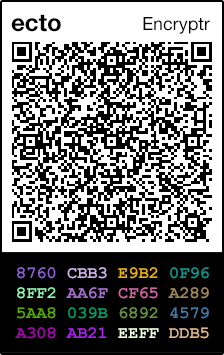
\includegraphics[width=0.25\textwidth]{id-card-border.png}
  \caption{Identity Card Example}
\end{figure}

\subsection{Identity Cards}
Crypton's peer verification mechanism also includes an effort
to create new metaphors in privacy-centered applications. Instead of teaching
users about public key cryptography, we wanted to find a metaphor that everyday
users will easily understand.

Crypton clients are expected to implement a Card generation class. This class
will take an Account object as input and output an image with username, application
name, colorized fingerprint, and a QR code. It is also expected to provide a method
taking a QR code-containing image as input to verify to peer automatically.

Rather than send a textual fingerprint to another user, Crypton applications
utilizing multi-user features are expected to generate and send a Card out of band
for consistency and the propagation of an understandable metaphor. These applications
are also expected to display a client-generated Card of the other party for verification.

\subsubsection{QR Code}
QR codes were chosen for their ubiquity and machine-readable properties. When
Bob receives Alice's ID Card out of band, he can simply load it into a
Crypton-enabled application and let his device verify the parity of the fingerprints.
Data in the QR code is encoded with JSON and contains the fields found in Table III.

\begin{table}[h]
\caption{Identity Card QR Fields}
\centering
\begin{tabular}{l l}
\hline\hline
\\ [0.1ex]
Name & Definition \\
\\ [0.1ex]
\hline
\\ [0.3ex]
version & version of this data structure \\
username & username of peer \\
fingerprint & \(fingerprint\) of user's public keys  \\
application & name of application which generated this card \\
signature & signature of fingerprint, \\
  & \ \ proving the user has access their private key \\
\\ [0.3ex]
\hline
\end{tabular}
\label{table:nonlin}
\end{table}

\subsection{Colorized Fingerprint}
For users who wish to verify the fingerprint manually, it is presented on the
bottom of the Card as a series of two-octet sections (for readability). The
sections are assigned a hexadecimal color by taking their first octet for the
red value, second octet for the green value, and the first octet of the next section
for their blue value - this provides cascading errors which further draw the user's
attention to discrepancies. Colorization is not to be relied upon as a verification
mechanism. It is only to make it easier to identify differences in the content of the fingerprint.

\section{Threat Model}
\subsection{Assumptions}
Crypton has initially been developed in JavaScript. However, there are no
apparent difficulties in porting its concepts to another language.
In its use of JavaScript, it could be easily assumed that Crypton was meant to
be used in a web browser. This is incorrect. Browsers are beset by a problem of
unverifiable code delivery in that users cannot verify that the script they received
from the server is as intended. Therefore, it is only recommended to use
Crypton in packaged applications. Tools such as Cordova\cite{cordova} or
node-webkit\cite{nodewebkit} are
used for packaging Crypton applications using the JavaScript client.
Clients implemented on disparate platforms are also expected to be distributed
in a packaged manner.

\subsection{Strengths}
Crypton at its core provides a cryptosystem meant to protect users' data,
share that data with other users, and send messages directly between users.
This is all meant to happen with the server having no knowledge about the content
of these messages or data containers. Furthermore, with the use of HMACs as public 
container names, the server's knowledge of application metadata is hindered.

In the use of SRP for authentication, without storing a password equivalent,
data compromise in a server breach is limited if not negligible. Without a user's
password, the only effective attack on that user's data would be to bruteforce
AES keys.

\subsection{Threats}
There are several problems which Crypton is not designed to mitigate.
In the event of a server compromise, the following threats to a Crypton system
are applicable:

\subsubsection{Traffic storage}
IP addresses or hostnames belonging to those accessing the server may be stored
by a malicious server operator or attacker, reducing the pseudoanonymity afforded
to users of a Crypton system (email addresses are not required for account generation).
This can be mitigated by accessing the server with Tor\cite{tor} or a similar system.

\subsubsection{Peer graph analysis}
Usernames are stored in plaintext by the server. Database records can be analyzed
to connect sharing and message networks between usernames. If this is used in
concert with traffic storage, the identities of a Crypton application's users may
be compromised.

\subsubsection{Container access frequency analysis}
Certain containers, such as the Trust State Container, are created, accessed, or
updated in a deterministic manner. A sophisticated attack may disclose
the identity of certain containers to narrow a bruteforce decryption attack.
This can be limited by choosing a strong password.

\section{Future Work}

\subsection{Container Compaction}
As containers are used over time, many records may be added to them. In order to
load a container, all of these records must be decrypted and parsed by the client.
As a result, loading a container will grow slower over the course of its lifetime
if it is constantly updated.

Container compaction would add a new transaction chunk type, which, when provided with
the ultimate desired state of the container (and barring transactional conflicts),
would remove all past records for that container and leave only the latest state.
This would decrease load times for heavily used containers significantly.

"Autocompaction" is also an interesting avenue to pursue, where compaction would occur
automatically upon saving a container. This would be useful for applications which
do not care to save historical versions of their data structures.

\subsection{Container caching}
Another improvement to container load times would be to cache encrypted container
records locally and sync them with what the server provides. This will require the
addition of event emission and perhaps Operational Transformations to the Container
class in order to work safely.

\subsection{Multiple Client Implementations}
The JavaScript client was developed as a reference implementation. The cryptosystem
is sufficiently abstracted so that it may be implemented on most platforms. This
will be most easily acheived by implementing a core client in C. Wrappers may be
written in Objective-C, Java, etcetera to provide syntactic sugar and
platform-idiomatic APIs.

\subsection{Hosted Backend}
A service is being developed to host back-end Crypton servers. This means there
will only be front-end development work for someone wishing to build a Crypton
application.

\section{Conclusion}
Today's application developers have the responsibility to protect their users' data.
We have seen in the recent past where SSL did not protect users\cite{SSLImpersonation}
making it an imperfect solution for online data security. End-to-end encryption
technology, frameworks and services are the best hope for a truly private application
development environment. Crypton's approach is an attempt at filling this gap in the
marketplace. While Crypton cannot solve all data security problems we have today, it is
a good start in the direction of allowing developers without a concentration in
cryptography a framework that keeps application data private.

It is too much to ask all developers interested in building applications that are
centered on privacy to become proficient in cryptographic primitives and their
use in secure cryptosystems. This being the case, Crypton is a small step
toward a more private application development future.

The chief concern of Crypton is the user experience from developer APIs
all the way up to the user interface end users operate for key exchange. With the
cryptography hidden from the developer and new metaphors like "ID cards" to replace
"key exchange", the authors think the way is paved toward every developer having
the ability to create simple, secure, and private applications.

Whether you utilize Crypton or not, the authors implore you to protect yourself
and your users from adversaries by encrypting all data, not only on the wire but
at rest.

\section*{Acknowledgment}
The authors would like to thank Alan Fairless and David Zuwenden for creating the
original Crypton specification, Tommy Williams for incredible API feedback and
early application work, Chip Black for work on SRP implementation, and Tomas
Touceda for internal security reviews.

\newpage
%\onecolumn
\begin{thebibliography}{14}
%\bibitem{spying} \url{https://www.eff.org/nsa-spying}
\bibitem{spying} Greenwald, Glenn. "NSA Collecting Phone Records of Millions of Verizon Customers Daily." 5 June 2013. \url{http://www.theguardian.com/world/2013/jun/06/nsa-phone-records-verizon-court-order}
\bibitem{defenseindepth} "Defense In Depth." National Security Agency. \url{https://www.nsa.gov/ia/_files/support/defenseindepth.pdf}
\bibitem{SRP} Wu, T. "The SRP Authentication and Key Exchange System." The Internet Engineering Task Force, Sept. 2000. \url{https://www.ietf.org/rfc/rfc2945.txt}
\bibitem{sjcl} Stark, Emily, Michael Hamburg, and Dan Boneh. "Symmetric Cryptography in Javascript." Computer Science Department, Stanford University. \url{https://crypto.stanford.edu/sjcl/acsac.pdf}
\bibitem{cryptojs} Mott, Jeff. "Crypto-js." \url{https://code.google.com/p/crypto-js/}
\bibitem{mylar} "Mylar." MIT CSAIL Computer Systems Security Group. \url{http://css.csail.mit.edu/mylar/}
\bibitem{mylarpaper} Pope, Raluca Ada, Emily Stark, Jonas Helfer, Steven Valdez, Nikolai Zeldovich, M. Frans Kaashoek, and Hari Balakrishnan. "Building Web Applications on Top of Encrypted Data Using Mylar." MIT CSAIL Computer Systems Security Group, Meteor Development Group. \url{http://css.csail.mit.edu/mylar/mylar.pdf}
\bibitem{endtoendblog} Somogyi, Stephan. "Making End-to-end Encryption Easier to Use." Google Online Security Blog. Google, 3 June 2014. \url{http://googleonlinesecurity.blogspot.com/2014/06/making-end-to-end-encryption-easier-to.html}
\bibitem{endtoend} "end-to-end." Google. \url{https://code.google.com/p/end-to-end/}
\bibitem{endtoendkeydistribution} "end-to-end Key Distribution." Google. \url{https://code.google.com/p/end-to-end/wiki/KeyDistribution}
\bibitem{gcm} Dworkin, Morris. "Recommendation for Block Cipher Modes of Operation: Galois/Counter Mode (GCM) and GMAC." National Institute of Standards and Technology. Nov. 2007. \url{http://csrc.nist.gov/publications/nistpubs/800-38D/SP-800-38D.pdf}
\bibitem{elgamal} Elgamal, Taher. "A Public Key Cryptosystem and a Signature Scheme Based on Discrete Logarithms." IEEE Transactions on Information Theory IT-31.4 (1985). \url{http://caislab.kaist.ac.kr/lecture/2010/spring/cs548/basic/B02.pdf}
\bibitem{ecdsa} "Digital Signature Standard." National Institute of Standards and Technology, July 2013. \url{http://nvlpubs.nist.gov/nistpubs/FIPS/NIST.FIPS.186-4.pdf}
\bibitem{curves} "Recommended Elliptic Curves for Federal Government Use." National Institute of Standards and Technology, July 1999. \url{http://csrc.nist.gov/groups/ST/toolkit/documents/dss/NISTReCur.pdf}
\bibitem{srp-protocol} "SRP Protocol Design." Stanford University. \url{http://srp.stanford.edu/design.html}
\bibitem{pbkdf2} Kaliski, B. "PKCS \#5: Password-Based Cryptography Specification." The Internet Engineering Task Force, Sept. 2000. \url{https://tools.ietf.org/html/rfc2898}
\bibitem{cordova} "Cordova." Apache. \url{https://cordova.apache.org/}
\bibitem{nodewebkit} Wang, Roger. "node-webkit". \url{https://github.com/rogerwang/node-webkit}
\bibitem{tor} "The Tor Project". Tor. \url{https://www.torproject.org/about/corepeople.html.en}
\bibitem{SSLImpersonation} Goodin, Dan. "In the Wild: Phony SSL Certificates Impersonating Google, Facebook, and ITunes." Ars Technica, 12 Feb. 2014. \url{http://arstechnica.com/security/2014/02/in-the-wild-phony-ssl-certificates-impersonating-google-facebook-and-itunes/}
\end{thebibliography}
\end{document}

